%---------------------------------------------------------------------------------
\chapter{Method for OFDM Timing Synchronisation}
\label{chap:Synchronisation}
%---------------------------------------------------------------------------------

%---------------------------------------------------------------------------------
\section{Introduction}
%---------------------------------------------------------------------------------
OFDM performance is sensitive to receiver synchronisation \cite{Hanzo2006}.
Frequency offset causes inter-subcarrier interference, and errors in timing synchronisation can lead to inter-symbol interference.
Therefore, accurate synchronisation is critical to the performance of OFDM systems.
This section summarises conventional synchronisation methods used with OFDM, discussing their merits and drawbacks, before the following sections present a new and efficient method that is robust to large frequency offset, obtains accurate  and robust synchronisation and requires relatively low computational complexity. In particular, it is designed to be suitable for hardware implementation on reconfigurable systems.

The method presented in this chapter has also been discussed in:
\begin{itemize}
\item T. H. Pham, I. V. McLoughlin, and S. A. Fahmy, ``Robust and Efficient OFDM Synchronisation for FPGA-Based Radios,'' in \textit{Circuits, Systems, and Signal Processing, vol. 33, no. 8, pp. 2475 - 2493, Aug. 2014, Springer}~\cite{Pham2014}.
\end{itemize}

%---------------------------------------------------------------------------------
\section{Related Work}
%---------------------------------------------------------------------------------
Autocorrelation-based methods are commonly chosen for implementing synchronisation because of their low computational complexity. In \cite{Schmidl1997}, timing metrics are defined as follows, beginning with the normalised power measure \emph{M[d]}:

\begin{center}
\begin{equation}
\label{MMetric}
M[d] = \frac{|P[d]|^2} {(R[d])^2},
\end{equation}
\end{center}

where $d$ denotes a time index corresponding to the first sample in a search space comprising $2L$ samples of received signal $r$. The power measure \emph{R}, which represents the energy of the second half of the receiver search window, is defined as:

\begin{center}
\begin{equation}
\label{RMetric}
R[d] =\sum_{m =0}^{L-1}   |r[d+m+L]|^2,
\end{equation}
\end{center}

and the normalisation parameter \emph{P} computes the correlation between two periodic halves in the search window as:

\begin{center}
\begin{equation}
\label{PMetric}
P[d] =\sum_{m =0}^{L-1}    (r^{*}[d+m] r[d+m+L] ),
\end{equation}
\end{center}

%where superscript \textquotedblleft$*$\textquotedblright  denotes complex conjugation.

The metric \emph{M[d]} is illustrated for a typical channel in Fig.~\ref{fig:M1-10dB}, where it can be seen to form a distinct plateau in the region when the preamble is presented within a received window.
Clearly, \emph{M[d]} accurately detects the preamble, however the nature of the plateau having a flat top presents an uncertainty in terms of exact positioning, and hence reduced accuracy in determining the exact start of the frame, compared to a metric which peaks.

\begin{figure}
	\centerline{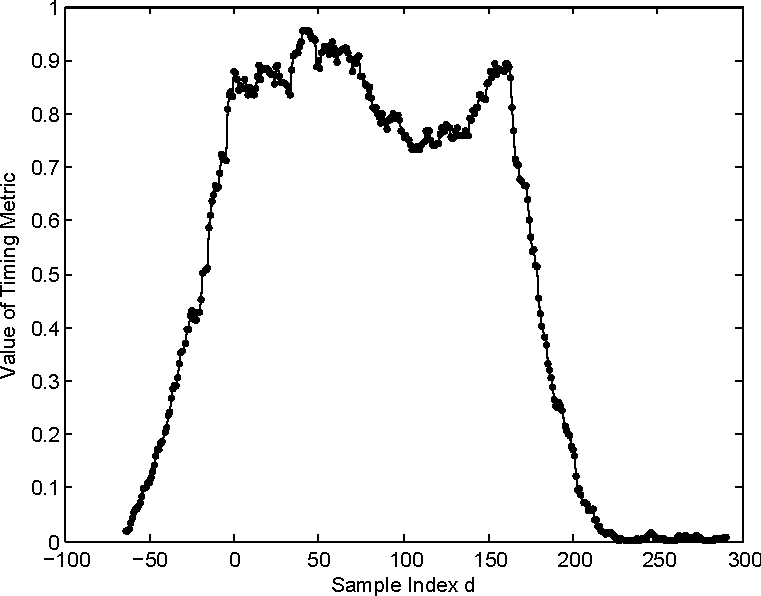
\includegraphics [width=0.8\columnwidth] {figures/M1_10dB.pdf} }
	\caption{The timing metric in \cite{Schmidl1997} applied to the IEEE~802.16-2009 preamble in an AWGN channel (SNR = 10dB)}
	\label{fig:M1-10dB}
\end{figure}

In order to improve the accuracy of synchronisation, a scheme is often used as in \cite{Schwoerer2002,Manavi2004,Guffey2007,Huang2010,Recio2010} based on combining the above metric for detecting the frame, estimated coarse STO and fractional CFO, and additional cross-correlation operations for computing fine STO and integer CFO as we will explore below.

%---------------------------------------------------------------------------------
\subsection{Coarse STO and Fractional CFO Estimation}
%---------------------------------------------------------------------------------

First, the plateau of the \emph{M[d]} metric is used to detect a frame start and estimate coarse STO by comparing the magnitude of \emph{M[d]} to a given threshold. After this, the CFO is estimated using the \emph{P} metric in (\ref{PMetric}).
We now assume that we are receiving a signal \emph{s[d]} which has a normalised carrier frequency offset $\xi$ with respect to \emph{r[d]}:
\begin{center}
\begin{equation}
\label{freoffsignal}
s[d] =  e^{j2\pi\xi \frac{d}{N}}*r[d].
\end{equation}
\end{center}
where \emph{N} is the numbers of subcarriers of the OFDM symbol. At the plateau of \emph{M[d]}, the received samples in the window will be periodic:
\begin{center}
\begin{equation}
\label{signalperiodic}
r[d] =  r[d+L].
\end{equation}
\end{center}

Substituting (\ref{freoffsignal}) and  (\ref{signalperiodic}) in (\ref{PMetric}) we find that

\begin{eqnarray}
\label{PMetricfreoffset}
P[d] &=& \sum_{m =0}^{L-1}  (s^{*}[d+m] s[d+m+L] ) \nonumber \\
 &=& e^{j2\pi \xi \frac{L}{N}} \sum_{m =0}^{L-1}  |r[d+m]|^2
\end{eqnarray}
The CFO can be determined as follows;
\begin{equation}
\label{fractionalCFO}
\xi = \frac{\angle P[d] + 2\pi z}{2\pi \frac{L}{N}}
\end{equation}
where  $\angle P[d]$ is the angle of \emph{P[d]} within the range -$\pi$ to $\pi$.
The CFO consists of 2 parts: the fractional part, $\hat{\lambda} = \frac{\angle P[d]}{2\pi \frac{L}{N}}$, can be estimated replied on $\angle P[d]$ and the integer part (IFO) is represented by an integer \emph{z}, $\hat{\epsilon} = \frac{z N}{L}$.
The fractional CFO estimation has a range limitation as follows:
\begin{eqnarray}
\label{fractionalCFOlimitation}
 -\frac{N}{2L} & <  \hat{\lambda}   < & \frac{N}{2L}
\end{eqnarray}

Clearly, the range over which fractional CFO can be estimated may be increased by decreasing the length of period \emph{L}.
However, because of the influence of channel noise, a smaller \emph{L} would also degrade the accuracy of estimation of the fractional CFO $\hat{\lambda}$.
In the case of the IEEE~802.16-2009 preamble~\cite{IEEE80216}, the number of subcarriers \emph{N} and length of period \emph{L} are commonly chosen to be 512 and 64 samples respectively \cite{Kim2008}.
Hence the fractional CFO estimation range is limited to within -2 to +2 subcarrier spacings. Meanwhile, the value of IFO parts $\hat{\epsilon}$ is estimated as an integer multiple of 4.

The method outlined above is fast and robust for estimating coarse STO and fractional CFO.
However it has some drawbacks.
First, the coarse STO is estimated by comparing the metric to a threshold.
It is not certain that the samples for estimating the fractional CFO are within the plateau of \emph{M[d]} in which the received samples in the window will be periodic.
This degrades the performance of fractional CFO estimation.
Second, the CFO estimation can only be performed correctly in the limited range of the fractional CFO shown in (\ref{fractionalCFOlimitation}).
If the actual CFO lies outside this range, it is necessary to estimate the integer CFO separately.

%---------------------------------------------------------------------------------
\subsection{Fractional CFO Compensation}
%---------------------------------------------------------------------------------

Fine STO estimation, accomplished using cross-correlation, is sensitive to CFO.
Thus the estimated fractional CFO must first be used for frequency offset compensation.
This is done by phase de-rotating the received samples in the time domain:

\begin{eqnarray}
\label{comfreoffsignal}
\widehat{r[d]} =  e^{-j2\pi\xi \frac{d'}{N}}*s[d];  & d' = d + \mathit{t_{off}}.
\end{eqnarray}

$\widehat{r[d]}$ and \emph{s[d]} are the compensated samples and frequency offset samples, respectively. \emph{d'} is the coarse estimated timing index that differs from the correct timing index $\mathit{t_{off}}$ samples.
Substituting (\ref{freoffsignal}) in (\ref{comfreoffsignal}), we get:

\begin{eqnarray}
\label{phaseerror}
\widehat{r[d]} &=&  e^{-j2\pi\xi \frac{(d+t_{off})}{N}}*e^{j2\pi\xi \frac{d}{N}}*r[d] \nonumber \\
&=& e^{-j2\pi\xi \frac{t_{off}}{N}}*r[d].
\end{eqnarray}

When compensating the fractional CFO, the fine STO has still not been estimated. This results in a common phase error within the coarse CFO compensated samples as shown in (\ref{phaseerror}).

%---------------------------------------------------------------------------------
\subsection{Fine STO Estimation}
%---------------------------------------------------------------------------------

The purpose of timing synchronisation is to find the correct starting point for receiver demodulation.
This starting point will generally mark the beginning of a discrete Fourier transform (DFT) window.
Coarse time synchronisation is commonly based on auto-correlation as mentioned above, leading to relatively simple hardware implementation.
However, with purely coarse STO, it is almost impossible to achieve sufficient accuracy to correctly detect the starting point.
Thus,  fine STO estimation is necessary to refine the accuracy of timing synchronisation.
To obtain more accurate fine STO estimation, cross-correlation is usually performed between the received samples and known transmitted preamble.
The peak cross-correlation occurs when the received samples match the known preamble.
Fine STO can thus be found by locating this peak within a search window.
In order to reduce the overhead of cross-correlation, a sign bit multiplier can be used instead of a real multiplier to calculate cross-correlation. However, this is much more sensitive to CFO in practice \cite{Schwoerer2002}. Some researchers employ enhanced methods based on cross-correlation for the time synchronisation.
For example, Kishore and Reddy \cite{Kishore2006} presented an algorithm using cross-correlation between the known transmitted and received preamble symbols.
The timing metrics for synchronisation using this method perform the normalised \emph{M[d]} calculation, and use the same denominator \emph{R} as in (\ref{MMetric}) and (\ref{RMetric}), however they refine the numerator \emph{P} as follows;
\begin{center}
\begin{equation}
\label{PKishore}
P[d] =\sum_{m =0}^{L-1}    (r[d+m] a[m])^{*} (r[d+m+L] a[m]),
\end{equation}
\end{center}
where $d$ again denotes the time index corresponding to the first sample in a window of \emph{2L} samples of received signal $r$ and superscript \textquotedblleft$*$\textquotedblright again denotes complex conjugation. In (\ref{PKishore}) the samples $a$ are now the known, transmitted, time domain preamble samples.

The cross correlation now produces distinct peaks at the times when received samples match the known transmitted samples of the preamble. Fig.~\ref{fig:M2-10dB} illustrates this by plotting \emph{M} versus the sample index $d$ for an example channel in AWGN with SNR~=~10{\thinspace}dB.
A frame is detected when \emph{M} crosses a threshold and the start of frame is found by searching the peaks of \emph{M}.
This can accurately determine the start of frame even at low SNRs.
Moreover, this method is robust to large CFO for time synchronisation.
Simulations \cite{Kishore2006} show that time synchronisation can be performed effectively with CFO~=~10.5 subcarrier spacings.
However, the cross-correlation operation requires complex computation.
Although the complexity of cross-correlation can be reduced using multiplierless correlation \cite{Yip2003}, the multiplierless correlator degrades the precision of metric \emph{P}, used for estimating frequency offset.
In general, this method is appropriate for time synchronisation but requires significant hardware resources for implementing the cross-correlation.

\begin{figure}
	\centerline{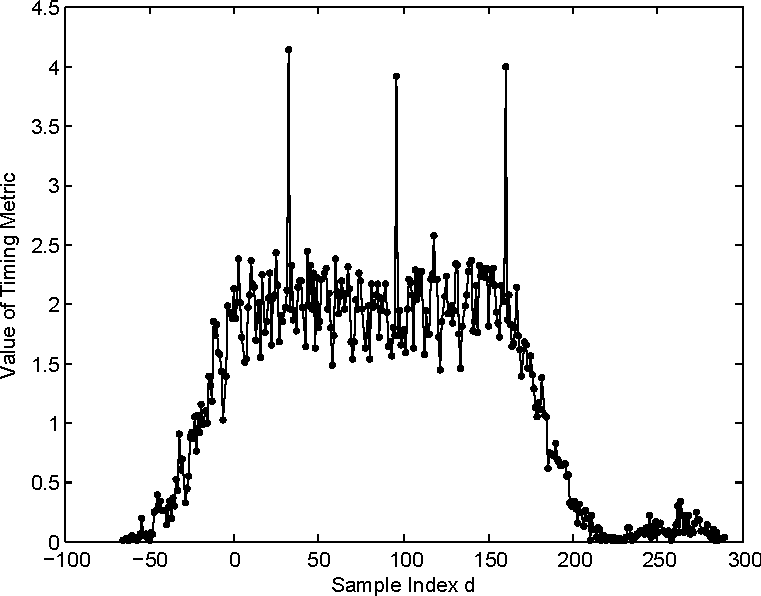
\includegraphics [width=0.8\columnwidth] {figures/M2_10dB.pdf} }
	\caption{The timing metric in \cite{Kishore2006} applied to the IEEE~802.16 preamble in an AWGN channel (SNR = 10dB)}
	\label{fig:M2-10dB}
\end{figure}

%---------------------------------------------------------------------------------
\section{Proposed Fractional CFO Estimation and Synchronisation}
%---------------------------------------------------------------------------------

Considering the limitations of previous work, we propose new timing metrics to take advantage of preamble characteristics such as period and energy distribution.
Again, the proposed method is illustrated for the specific case of the IEEE~802.16-2009 preamble, as shown in Fig.\ref{fig:SyncFlow}.

Firstly, we define the autocorrelation between the two halves of the receiver window for normalisation purposes;

\begin{equation}
\label{ProposedP}
P'[d] =\sum_{m =0}^{C-1}    (r^{*}[d+m] r[d+m+L] )
\end{equation}

where $d$ denotes a time index of received signal $r$ that now corresponds to the first sample in a window of \emph{L+C} samples of received signal, \emph{L} being the length of preamble period (64 for the IEEE802.16 preamble) and \emph{C} being the length of received samples for estimation, respectively.

Next, a power measure, \emph{R'} is proposed which takes account of both received and transmitted symbol power;

\begin{equation}
\label{ProposedR}
R'[d] =\sum_{m =0}^{C-1}   |r[d+m+L]|^2  |a[m]|^2
\end{equation}


\begin{figure}
\centering
	\begin{tikzpicture}
	\begin{axis}[ xlabel= Sample index d, ylabel= Value of Timing Metric, legend columns=3,	legend style={at={(0.5,1.02)}, anchor=south, cells={anchor=west}, draw=none}, x post scale=1.4]
		\addplot+[black, style={densely dashed, color=violet, thick}, every mark/.append style={mark=none}]  table [x index=0, y index=1] {./Dat/Pp_Rp.dat};
		\addlegendentry{P' Metric};
		\addplot+[black, style={solid, color=red, thick}, every mark/.append style={mark=none}]	 table [x index=0, y index=2] {./DAT/Pp_Rp.dat};
		\addlegendentry{R' Metric};
	\end{axis}
	\end{tikzpicture}
	\caption{Proposed timing metrics applied to the IEEE~802.16 preamble in AWGN (SNR = 10{\thinspace}dB, CFO = 10.5).}
	\label{fig:ProposedMetric-10dB}
\end{figure}


In common with the metric developed by Schmidl and Cox \cite{Schmidl1997}, our proposed \emph{P'[d]} detects the periodic characteristic of the preamble and can thus be used for estimating fractional CFO.
\emph{P'} forms a plateau as evident in Fig.\ref{fig:ProposedMetric-10dB} when the preamble is present within the receiver window.
\emph{R'} is then used to find the starting point of the preamble based on its energy distribution.
\emph{R'} causes peaks shown in Fig.\ref{fig:ProposedMetric-10dB} at the point where the energy distribution of the received samples matches that of the transmitted preamble.
Since the \emph{R'} metric that is used to estimate time synchronisation is computed on the square of the amplitude of received samples, the time synchronisation is insensitive to the CFO that effects the phase of the received samples.
Moreover, computing on amplitude squared, a real number, requires less resources than using complex numbers as in alternative approaches such as \cite{Kishore2006}.
In addition, the time synchronisation is performed based on the peak value of \emph{R'} rather than its absolute value.
Therefore, \emph{R'} is a good candidate for implementation using a multiplierless correlator to reduce computational complexity.
\begin{figure}
	\centerline{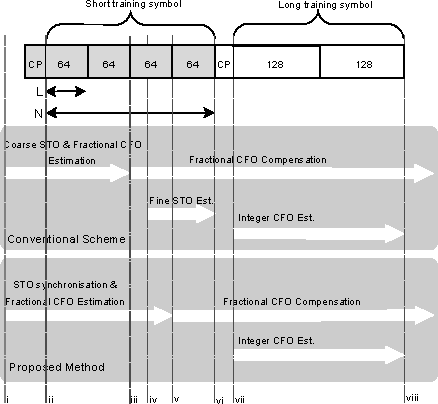
\includegraphics [width=1\columnwidth] {figures/SynFlow_IVMannotated.pdf}}
	\caption{The synchronisation flow according to the received samples within the preamble showing its packet format above the conventional synchronisation scheme flow (middle), and proposed scheme (bottom). With the packet timing illustrated above.}
	\label{fig:SyncFlow}
\end{figure}
Fig.\ref{fig:SyncFlow} illustrates the flow of the proposed synchronisation method according to the received samples of the preamble, compared to that of the conventional scheme.
As can be seen in the conventional scheme, the coarse STO and fractional CFO estimation are performed in the two first periods of the short training symbol from (i) to (iii), and then the estimated fractional CFO is used for compensation.
The fine STO is estimated in the last period of the short training symbol from (iv) to (vi), and integer CFO should be computed in the long training symbol from (vii) to (viii).
By contrast, the proposed method performs STO synchronisation and fractional CFO estimation in the three first periods of the short training symbol from (i) to (iv), and the start of frame will be detected at (ii).
Then, the fractional CFO compensation is computed, and integer CFO estimation is performed in the long training symbol from (vii) to (viii).

The method used for synchronisation based upon these metrics is described in the following sub-sections.

\subsection{Frame Synchronisation and Fractional CFO Estimation}

First, frame detection is performed by comparing the metric \emph{P'} to \emph{R'} with a threshold \emph{thr} as shown in (\ref{framedetection})
\begin{equation}
\label{framedetection}
|P'[d]| > thr * R'[d].
\end{equation}

%The threshold is different for each channel and needs to be determined empirically by simulation (in common with other systems such as \cite{Kishore2006}).
Fig.\ref{fig:TimeSyn_thr_AWGN} shows the performance of the frame synchronisation in the given channel for different threshold values.
With each threshold value, 1000 frame detections are simulated.
\begin{figure}
	\centerline{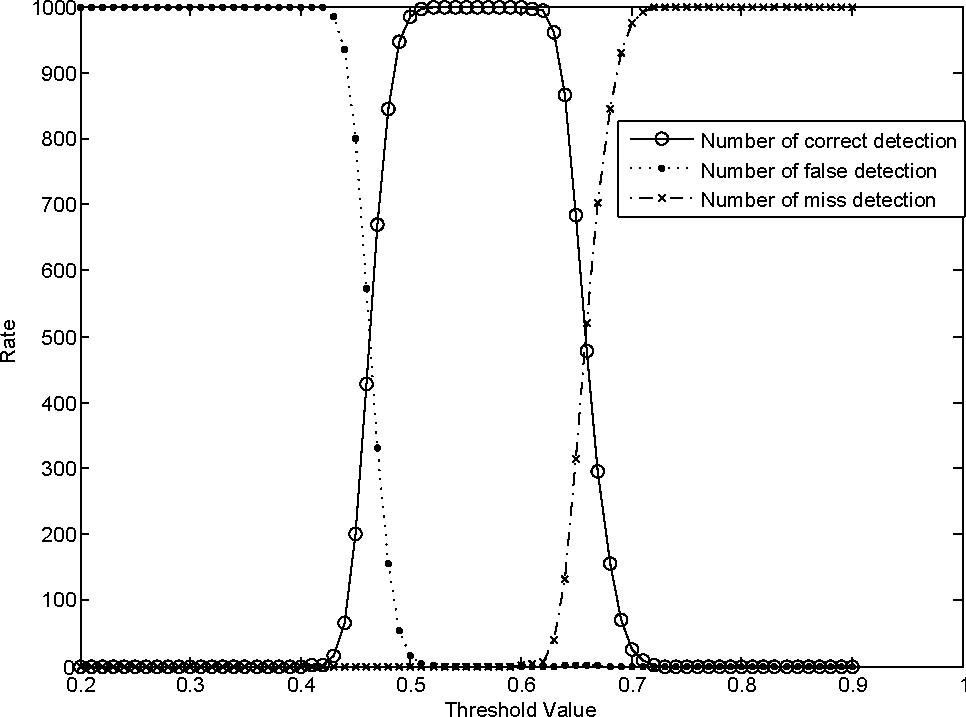
\includegraphics [width=0.9\columnwidth] {figures/ThresholdEffect.pdf}}
	\caption{Performance of the frame synchronisation method versus the selection threshold for an AWGN channel (with SNR =10dB).}
	\label{fig:TimeSyn_thr_AWGN}
\end{figure}
The number of correct detections indicates how often the time synchronisation has been found correctly at the start of the frame, while the number of false detections indicate that the time synchronisation gets the wrong start of the frame.
Otherwise, the frame is not detected (i.e. $|P'[d]|$ can be not greater than $thr * R'[d]$), and a miss detection is declared.
From the results plotted,  the optimum value can be seen to be around 0.55.
If the threshold is too small, noise may cause a failure of detection.
On the other hand, when the threshold is large, the frame detection may be missed if the noise reduces the amplitude of the timing metric, which consequentially does not cross the threshold.
The threshold values depend on the operating channel and are determined empirically by simulation (in common with other systems such as in [36]). Assuming the set of possible channels is known, the thresholds for these channels can be pre-determined by simulation. The performance of synchronisation is evaluated with increased thresholds for a given channel model. The threshold value corresponding to the best performance is selected for the channel model. The determined threshold values are stored in a look-up table. Based upon current channel model and conditions, a threshold is selected from the look-up table.



After a frame is detected, the starting point of the short preamble is found by searching for the peaks in \emph{R'[d]}.
As can be seen in Fig. \ref{fig:ProposedMetric-10dB}, two peaks in \emph{R'[d]} will bracket the transition to the plateau in \emph{P'[d]} shown at sample indices of -31 and 33, respectively.
The second peak is used as the starting point for the DFT window.
This is accomplished for the maximum values of $R'[d] + R'[d - L]$ over the next \emph{L} samples after frame detection.
Second, the fractional CFO estimation is presented in (\ref{proposedfractionalCFO}) based on the \emph{P'[d]} metric similarly to other work such as \cite{Schmidl1997,Schwoerer2002,Manavi2004,Guffey2007,Huang2010,Recio2010};

\begin{equation}
\label{proposedfractionalCFO}
\hat{\lambda} = \frac{\angle P'[d]}{2\pi \frac{L}{N}}
\end{equation}
where $\hat{\lambda}$ is the estimated fractional CFO, $\angle P'[d]$ denotes the angle of \emph{P'[d]} and \emph{N} is the number of subcarriers.
In this proposed method, the fractional CFO is estimated at the starting point of the preamble to guarantee that the correct angle of \emph{P'[d]} is taken for estimation. Using the conventional techniques, the inherent uncertainty in the coarse STO does not allow this to be achieved in practice.
Thus, the estimated fractional CFO in the proposed method will, on average, tend to be more accurate.
In addition, this method separates the length of preamble period \emph{L} and the length of received samples for estimation \emph{C}, and because of that \emph{L} can be small to extend the range of fractional CFO, and \emph{C} can be longer to increase the robustness to channel noise. For the IEEE~802.16 preamble, \emph{C} is set equal to \emph{2L} to improve the overall precision of synchronisation.

\subsection{Fractional CFO Compensation}

Compensating the fractional CFO is performed in the traditional way by phase de-rotating the received samples in the time domain;

\begin{eqnarray}
\label{proposedcomfreoffsignal}
\widehat{r[d]} &=&  e^{-j2\pi\Delta f_{c}dT_{s}}*s[d]. \nonumber \\
&=&  e^{-j2\pi\xi \frac{d}{N}}*e^{j2\pi\xi \frac{d}{N}}*r[d] \nonumber \\
&=& r[d].
\end{eqnarray}
However, in this proposed method, the frame synchronisation is achieved before performing fractional CFO compensation, therefore, $t_{off}$ is removed, and thus, the common phase errors caused by fractional CFO compensation are missing.
The compensated received samples are then demodulated using the DFT to obtain the received symbols in the frequency domain.

%---------------------------------------------------------------------------------
\subsection{Simulation Results and Discussion}
%---------------------------------------------------------------------------------
In this section, we will evaluate the performance of the proposed synchronisation method, applied to the IEEE~802.16-2009 downlink preamble, in MATLAB under both AWGN channels as well as the more realistic SUI channels that are widely used in the research literature \cite{Kishore2006,Kim2008}.

The Stanford University Interim (SUI) channel model~\cite{V.ErcegJuly2003} is used to simulate a frequency selective channel and takes into account  many wireless channel effects including delay spread, Doppler spread, phase noise, and channel interference.
In addition, the value of metrics computed in MATLAB are later verified with corresponding values from the FPGA simulation, to ensure practical functional equivalence.

In total, 100,000 OFDM frames, preceded by noise with randomly seeded AWGN and followed by preamble and data symbols, are used to evaluate synchronisation performance for each method.
The proposed method is compared to the state of the art method, in terms of accuracy of both time synchronisation and fractional CFO estimation.
The performance of STO estimation is measured in terms of failure rate (\%), and the accuracy of CFO estimation is evaluated in terms of mean square error (MSE).
We separately evaluate the robustness of time synchronisation against large CFO for each method.
Three versions of the proposed approach are constructed by varying the length, \emph{C}, of received samples for estimation based on (\ref{ProposedP}). These are investigated to determine the tradeoff between accuracy and computational cost, with \emph{C} defined as follows in each case:
\begin{itemize}
\item \textit{Prop 1}: $C=L$
\item \textit{Prop 2}: $C=2L$
\item \textit{Prop 3}: $C=3L$
\end{itemize}
These are compared to the state of the art method (denoted as \textit{SoA}) \cite{Liu2009,Recio2010}, and the method of Kishore and Reddy \cite{Kishore2006} (denoted as \textit{K\&R}) for a number of evaluation scenarios.
First, the performance of each method is found for AWGN channels beginning with CFO = 0.5, then AWGN channels with CFO varying from -10 to +10 times carrier spacing, then SUI1, and finally SUI2 channels.

		\subsubsection{Performance in AWGN}
\begin{figure}[h]
\centering
    	\begin{tikzpicture}
	\begin{semilogyaxis}[ xlabel=SNR(dB), ylabel=Fail rate of frame synchronisation (\%), legend columns=3,	legend style={at={(0.5,1.02)}, anchor=south, cells={anchor=west}, draw=none},
						 xmax=16, ymin=0.001, ymax=100, x post scale=1.4]
		\addplot+[style={dashed, thick},every mark/.append style={mark=square, style=solid}] table [x index=0, y index=4] {./Dat/FailRate_AWGN.dat};
		\addlegendentry{ \textit{Prop3}};
		\addplot+[style={solid, thick},every mark/.append style={mark=diamond*, style=solid}] table [x index=0, y index=3] {./Dat/FailRate_AWGN.dat};
		\addlegendentry{ \textit{Prop2}};
		\addplot+[style={dotted, thick},every mark/.append style={mark=triangle, style=solid}] table [x index=0, y index=2] {./Dat/FailRate_AWGN.dat};
		\addlegendentry{ \textit{Prop1}};
		\addplot+[black, style={solid, thick},every mark/.append style={mark=*, style=solid}] table [x index=0, y index=1] {./Dat/FailRate_AWGN.dat};
		\addlegendentry{ \textit{SoA}};
		\addplot+[style={dashed, thick},every mark/.append style={mark=o, style=solid}]  table [x index=0, y index=9] {./Dat/FailRate_AWGN.dat};
		\addlegendentry{ \textit{K\&R}};
	\end{semilogyaxis}
	\end{tikzpicture}
\caption{Performance of time synchronisation in AWGN channels with a frequency offset of 0.5 subcarrier spacings.}
\label{fig:STO_AWGN}
\end{figure}

\begin{figure}[h]
\centering
    	\begin{tikzpicture}
	\begin{semilogyaxis}[ xlabel=SNR(dB), ylabel=MSE of Fractional CFO,  legend columns=3, legend style={at={(0.5,1.02)}, anchor=south, cells={anchor=west}, draw=none}, x post scale=1.4]
		\addplot+[style={dashed, thick},every mark/.append style={mark=square, style=solid}] table [x index=0, y index=4] {./Dat/Fest_AWGN.dat};
		\addlegendentry{ \textit{Prop3}};
		\addplot+[style={solid, thick},every mark/.append style={mark=diamond*, style=solid}] table [x index=0, y index=3] {./Dat/Fest_AWGN.dat};
		\addlegendentry{ \textit{Prop2}};
		\addplot+[style={dotted,thick},every mark/.append style={mark=triangle, style=solid}] table [x index=0, y index=2] {./Dat/Fest_AWGN.dat};
		\addlegendentry{ \textit{Prop1}};
		\addplot+[black, style={solid,thick},every mark/.append style={mark=*, style=solid}] table [x index=0, y index=1] {./Dat/Fest_AWGN.dat};
		\addlegendentry{ \textit{SoA}};
		\addplot+[style={dashed,thick},every mark/.append style={mark=o, style=solid}] table [x index=0, y index=5] {./Dat/Fest_AWGN.dat};
		\addlegendentry{ \textit{K\&R}};
	\end{semilogyaxis}
	\end{tikzpicture}
\caption{Performance of fractional frequency offset estimation in AWGN channels.}
\label{fig:Fest_AWGN}
\end{figure}

Fig.~\ref{fig:STO_AWGN} and  Fig.~\ref{fig:Fest_AWGN} plot the performance results of STO and CFO estimation in AWGN with a frequency offset of 0.5 subcarrier spacings, respectively.
\textit{SoA} and the proposed methods have much better performance than \textit{K\&R} in these tests, achieving perfect synchronisation when SNR exceeds 5{\thinspace}dB.
\textit{Prop1}'s STO estimation has slightly better accuracy with SNR below 3{\thinspace}dB but is worse at higher SNR than \textit{SoA}.
Increasing the length of received samples for estimation, i.e., setting $C = 2L$, allows \textit{Prop2} to obtain a remarkable improvement in STO estimation, clearly better than the estimation achievable by \textit{SoA}.
\textit{Prop3}, with $C = 3L$, demonstrates decreasing gains: it is not able to enhance accuracy as much as \textit{Prop2}, despite a considerable hardware cost incurred when increasing \emph{C}.
In addition, the CFO of \textit{Prop3} and \textit{Prop2} achieve significant improvement compared to the other methods in Fig.~\ref{fig:Fest_AWGN}, while the accuracy of \textit{Prop1} and \textit{SoA} are identical (the curve for \textit{Prop1} is hidden behind the curve for \textit{SoA} as a result).

The gap between \textit{Prop1} and \textit{Prop2} is much larger than that between \textit{Prop2} and \textit{Prop3}, again demonstrating decreasing gains as \emph{C} is extended. Thus, increasing \emph{C} from \emph{L} to \emph{2L} is a more effective improvement than extending \emph{C} from \emph{2L} to \emph{3L}.
The accuracy of CFO estimation in \textit{Prop2} is improved by about 5{\thinspace}dB in comparison to \textit{SoA} and \textit{K\&R}.
This improvement is as a result of the increased length of received samples for estimation, \textit{C}.
These results show the proposed method to be competitive with state of the art methods.

\subsubsection{Performance in Fading Channels}

\begin{figure}[h]
\centering
	\begin{tikzpicture}
	\begin{semilogyaxis}[ xlabel=SNR(dB), ylabel=Fail rate of frame synchronisation (\%), legend columns=3,	legend style={at={(0.5,1.02)}, anchor=south, cells={anchor=west}, draw=none},
						 xmax=16, ymin=0.5, ymax=100, x post scale=1.4]
		\addplot+[style={dashed,thick},every mark/.append style={mark=square, style=solid}] table [x index=0, y index=4] {./Dat/FailRate_SUI.dat};
		\addlegendentry{ \textit{Prop3}};
		\addplot+[style={solid,thick},every mark/.append style={mark=diamond*, style=solid}] table [x index=0, y index=3] {./Dat/FailRate_SUI.dat};
		\addlegendentry{ \textit{Prop2}};
		\addplot+[style={dotted,thick},every mark/.append style={mark=triangle, style=solid}]  table [x index=0, y index=2] {./Dat/FailRate_SUI.dat};
		\addlegendentry{ \textit{Prop1}};
		\addplot+[black, style={solid,thick},every mark/.append style={mark=*, style=solid}]  table [x index=0, y index=1] {./Dat/FailRate_SUI.dat};
		\addlegendentry{ \textit{SoA}};
		\addplot+[style={dashed,thick},every mark/.append style={mark=o, style=solid}]  table [x index=0, y index=9] {./Dat/FailRate_SUI.dat};
		\addlegendentry{ \textit{K\&R}};
	\end{semilogyaxis}
	\end{tikzpicture}
\caption{Frame synchronisation performance of various methods in an SUI1 channel with respect to SNR.}
\label{fig:STO_SUI1}
\end{figure}

\begin{figure}[h]
\centering
	\begin{tikzpicture}
	\begin{semilogyaxis}[ xlabel=SNR(dB), ylabel=Fail rate of frame synchronisation (\%), legend columns=3,	legend style={at={(0.5,1.02)}, anchor=south, cells={anchor=west}, draw=none},
 						 xmax=16, ymin=0.5, ymax=100, x post scale=1.4]
		\addplot+[style={dashed,thick},every mark/.append style={mark=square, style=solid}] table [x index=0, y index=8] {./Dat/FailRate_SUI.dat};
		\addlegendentry{ \textit{Prop3}};
		\addplot+[style={solid,thick},every mark/.append style={mark=diamond*, style=solid}] table [x index=0, y index=7] {./Dat/FailRate_SUI.dat};
		\addlegendentry{ \textit{Prop2}};
		\addplot+[style={dotted,thick},every mark/.append style={mark=triangle, style=solid}]  table [x index=0, y index=6] {./Dat/FailRate_SUI.dat};
		\addlegendentry{ \textit{Prop1}};
		\addplot+[black, style={solid,thick},every mark/.append style={mark=*, style=solid}]  table [x index=0, y index=5] {./Dat/FailRate_SUI.dat};
		\addlegendentry{ \textit{SoA}};
		\addplot+[style={dashed,thick},every mark/.append style={mark=o, style=solid}]  table [x index=0, y index=10] {./Dat/FailRate_SUI.dat};
		\addlegendentry{\textit{K\&R}};
	\end{semilogyaxis}
	\end{tikzpicture}
\caption{Frame synchronisation performance of various methods in an SUI2 channel with respect to SNR.}
\label{fig:STO_SUI2}
\end{figure}

Fig.~\ref{fig:STO_SUI1} and  Fig.~\ref{fig:STO_SUI2} present the performance results of STO estimation in SUI1 and SUI2 channels, respectively.
The proposed methods are seen to achieve much better accuracy than the \textit{K\&R} method.
Compared to \textit{SoA}, Fig.~\ref{fig:STO_SUI1} reveals that the estimation of \textit{Prop1}, \textit{Prop2} and \textit{Prop3} is more accurate when SNR is below 3{\thinspace}dB.
However, for higher SNRs, the accuracy of \textit{SoA} is slightly better than that of the proposed method.
Increasing the length of received samples for estimation achieves an improvement when SNR is below about 5{\thinspace}dB, although the results for \textit{Prop1}, \textit{Prop2} and \textit{Prop3} saturate and become almost identical at higher SNRs, as does \textit{K\&R}.

		\subsubsection{Performance with Large Frequency Offset}

\begin{figure}[h]
\centering
	\begin{tikzpicture}
	\begin{semilogyaxis}[ xlabel=SNR(dB), ylabel=Fail rate of frame synchronisation (\%), legend columns=3,	legend style={at={(0.5,1.02)}, anchor=south, cells={anchor=west}, draw=none},
						 xmax=16, ymin=0.001, ymax=100, x post scale=1.4]
		\addplot+[style={dashed,thick},every mark/.append style={mark=square, style=solid}] table [x index=0, y index=8] {./Dat/FailRate_AWGN.dat};
		\addlegendentry{\textit{Prop3}};
		\addplot+[style={solid,thick},every mark/.append style={mark=diamond*, style=solid}] table [x index=0, y index=7] {./Dat/FailRate_AWGN.dat};
		\addlegendentry{\textit{Prop2}};
		\addplot+[style={dotted,thick},every mark/.append style={mark=triangle, style=solid}]  table [x index=0, y index=6] {./Dat/FailRate_AWGN.dat};
		\addlegendentry{\textit{Prop1}};
		\addplot+[black, style={solid,thick},every mark/.append style={mark=*, style=solid}]  table [x index=0, y index=5] {./Dat/FailRate_AWGN.dat};
		\addlegendentry{\textit{SoA}};
		\addplot+[style={dashed,thick},every mark/.append style={mark=o, style=solid}]  table [x index=0, y index=10] {./Dat/FailRate_AWGN.dat};
		\addlegendentry{\textit{K\&R}};
	\end{semilogyaxis}
	\end{tikzpicture}
\caption{Performance of frame synchronisation in an AWGN channel with uniform random frequency offset varying from -10 to 10 times carrier spacing, with respect to SNR.}
\label{fig:STO_AWGN_Fre}
\end{figure}

The proposed method is designed to work even with large frequency offsets.
Fig.~\ref{fig:STO_AWGN_Fre} explores performance over 100,000 tests where the frequency offset is chosen randomly (with uniform distribution) from -10 to +10 times the subcarrier spacing for each test, in an AWGN channel.
This experiment is specifically designed to investigate the robustness of STO estimation in large CFO conditions and shows that the proposed methods still maintain good performance. \textit{K\&R} exhibits some accuracy degradation, however, all methods are seen to outperform \textit{SoA}. The proposed methods are therefore seen to offer robustness of STO estimation against large CFO.
This robustness against large CFO is because the proposed metric is computed on magnitude values that are insensitive to phase errors.
CFO estimation is not evaluated here because large CFO estimation requires an integer CFO estimator that is investigated in the subsequent section.

In summary, simulation results show that \textit{Prop3} and \textit{Prop2} have better STO and CFO estimation accuracy compared to other methods.
\textit{Prop3} enjoys just a small improvement in terms of STO estimation compared to \textit{Prop2} but this improvement incurs a significant hardware cost because the length of received samples for estimation must increase from \emph{2L} to \emph{3L}.
Given the results described in this sub-section, \textit{Prop2} is selected as an implementation candidate in the subsequent sub-section, where the trade-off between accuracy and hardware cost is explored in more detail.

\subsection{Hardware Implementation}
This sub-section discusses the implementation of, and presents the hardware optimisation of, the proposed method in terms of word size. The target FPGA is a low-power Xilinx Spartan-6 XC6SLX45 device, with ISE 13.2 used to evaluate both hardware resource and power consumption.
The results illustrate the trade-off between hardware consumption and the accuracy of the proposed method.
The above sub-section already revealed that the performance of \textit{K\&R} is generally worse than the other methods, moreover it requires many complex multiply operations to compute the cross-correlation for the \emph{P} Metric. For this reason, \textit{K\&R} is not implemented, only the proposed method and \textit{SoA} are compared here, in terms of hardware resources, power consumption, and accuracy. As mentioned above we set  $C=2L$ since \textit{Prop2} consistently showed performance close to \textit{Prop3}, and significantly better than \textit{Prop1}. It  therefore offers a good balance between increased hardware cost and performance.

		\subsubsection{Implementation of Conventional Synchroniser}

First, let us consider a conventional synchroniser. We have implemented this as shown in Fig.~\ref{fig:Con-Sync}, following the efficient implementation methods presented in \cite{Manavi2004,Wang2004,Guffey2007,Liu2009}.
The \emph{P} and \emph{R} timing metrics in (\ref{PMetric}) and (\ref{RMetric}), respectively are computed using delay and summation, whilst a very efficient signed bit multiplier \cite{Schwoerer2002} is used to significantly reduce the computational overhead of the cross correlation for fine timing synchronisation.

\begin{figure}[h]
	\centerline{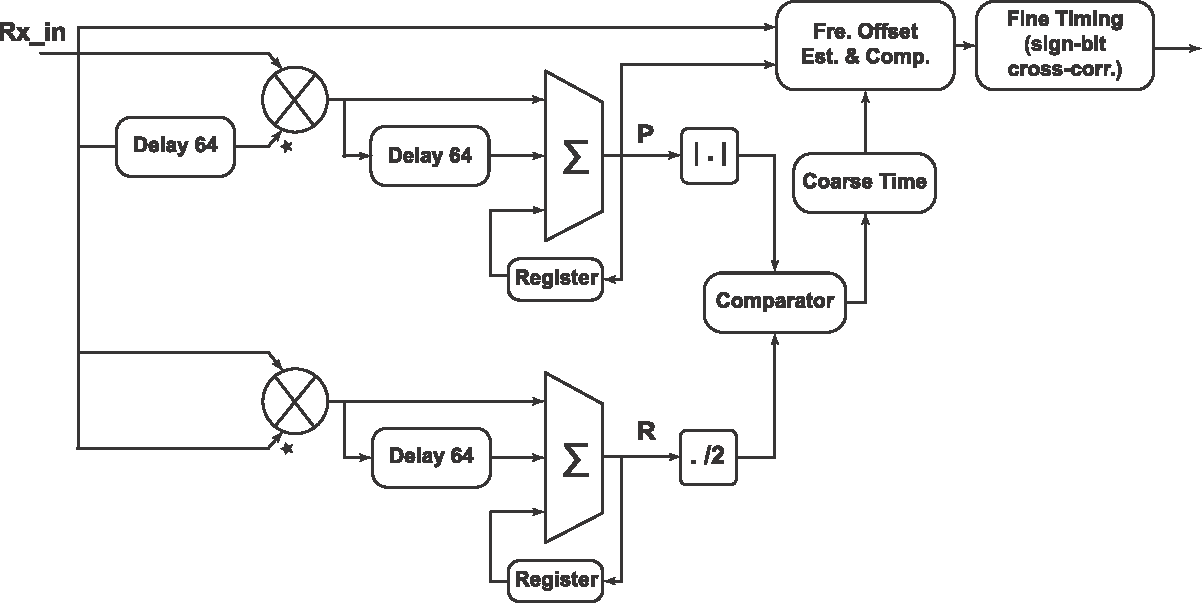
\includegraphics [width=0.8\columnwidth] {figures/Con_Sync.pdf}}
	\caption{Architecture of the conventional synchronisation FPGA implementation.}
	\label{fig:Con-Sync}
\end{figure}

We assume a 16-bit two's complement fixed point representation with 15 fractional bits (i.e. Q1.15 format in Q-notation).
The auto-correlation and squared amplitude of received samples are computed with a complex multiplier IP core that uses DSP slices.
Results are scaled to Q1.15 to reduce resource usage in subsequent pipeline stages.
Since this synchroniser is for the IEEE~802.16 preamble, the length of the delay is 64 samples.
Each element is scaled to be less than 1.0, guaranteeing that the final summation result is less than 64, needing just 7 bits for representation in two's complement.
Hence, the \emph{P} and \emph{R} values are represented in Q7.15 format.
For the $|P|$ metric, the auto-correlation uses a complex multiplier IP core to multiply the current received sample and the 64th delayed sample.
The magnitude of the \emph{P} metric is approximated to reduce hardware complexity as per \cite{Liu2009}.
For the \emph{R} metric, another complex multiplier is used to compute the squared magnitude of the received sample.
The threshold is commonly chosen to be 0.5, which can be implemented using a right shift by 1 bit \cite{Kim2008} instead of using a multiplier.
After the frame is detected, the \emph{P} metric is used to estimate and correct the fractional CFO.
A CORDIC IP core is used to determine the phase of the \emph{P} metric, and to derive the estimated fractional CFO.
The received samples are then compensated using phase accumulation and phase rotation.
These compensated samples are now used to determine fine timing synchronisation.

		\subsubsection{Implementation of Proposed Synchroniser}

\begin{figure}[h]
	\centerline{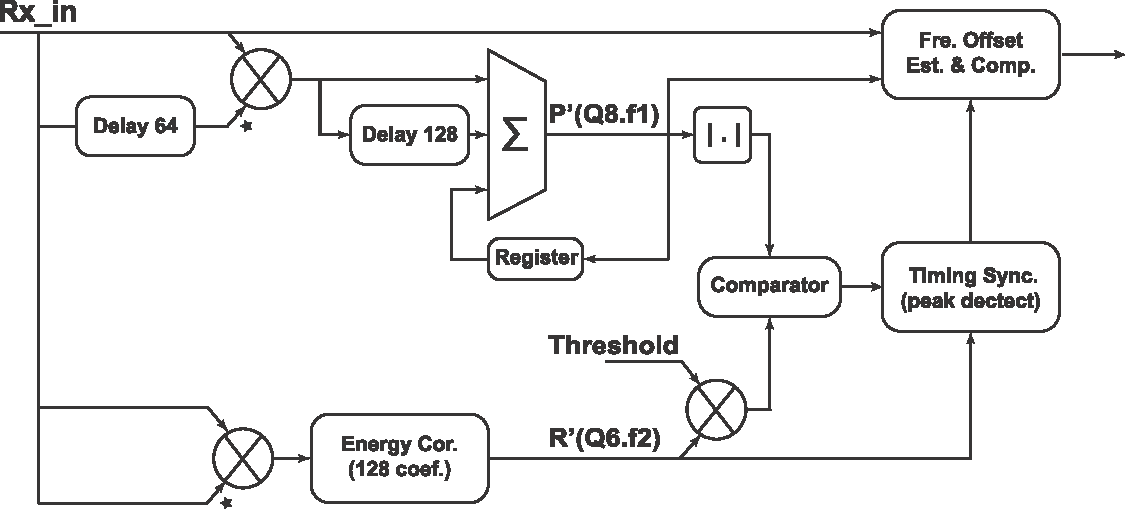
\includegraphics [width=0.8\columnwidth] {figures/Pro_Sync.pdf}}
	\caption{Architecture for the proposed synchronisation method implemented on FPGA.}
	\label{fig:Pro-Sync}
\end{figure}

The architecture for our proposed method is shown in Fig.~\ref{fig:Pro-Sync}.
The format of received samples is similar to the conventional design.
The \emph{R'} metric is determined using an energy correlator as illustrated in Fig.~\ref{fig:ML-Cor}.
The number of samples used to compute it is 128 and since the 128 samples of the short preamble are arranged in two identical spans of 64 samples each, the correlator only needs 64 taps.
The proposed method improves upon full cross-correlation not just by taking advantage of the periodic nature of the preamble, but also profiting from the real number computation of the proposed metrics, instead of requiring complex computation, and through enabling the use of a multiplierless correlator, yielding a significant computational saving.
Eqn.~(\ref{ProposedR-imp}) shows the derived equations of this optimisation:
\begin{eqnarray}
\label{ProposedR-imp}
R'(z) &=& I(z)A_{127} + I(z) z^{-1}A_{126} + ... + I(z) z^{-63}A_{64} \nonumber \\
	  &  &	+ I(z) z^{-64}A_{63} + ...+ I(z) z^{-127}A_0, \nonumber \\
	  &=& I(z)A_{63}   + I(z) z^{-1}A_{62}  +...+ I(z) z^{-63}A_0 \nonumber \\
	  &  &	+ I(z) z^{-64}A_{63} + ...+I(z) z^{-127} A_0], \nonumber \\
	  &=& (I(z)+I(z)z^{-64})A_{63} +... \nonumber \\
	  &  & 	+ (I(z)+I(z)z^{-64}) z^{-63}A_0, \nonumber \\
	  &=&I(z) (1+z^{-64})A_{63} +  z^{-1}(I(z)(1+z^{-64})A_{62}\nonumber \\
	  &	&						 + z^{-1 }( ...+z^{-1}I(z)(1+z^{-64})A_{0}))),
\end{eqnarray}
where \emph{I} is the squared amplitude of the received sample and $A_n$ denotes the normalised squared amplitude of known preambles.
Following this, a multiplierless correlator, as described in detail in \cite{Pham2012}, is used to compute the output, shown in block diagram form in Fig.~\ref{fig:ML-Cor}.

\begin{figure}[h]
	\centerline{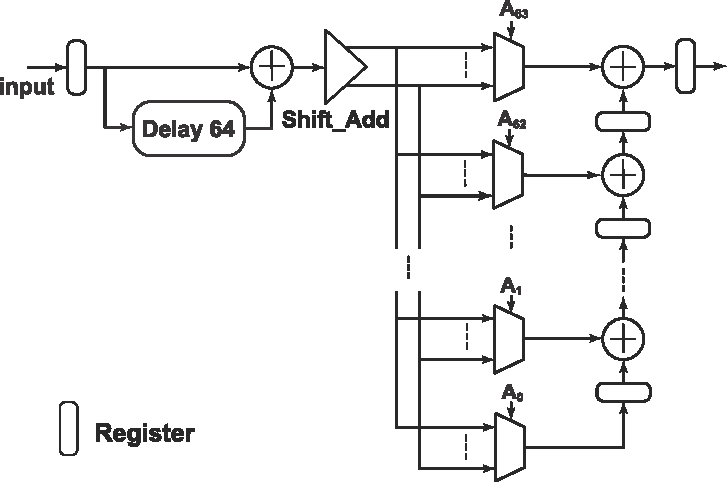
\includegraphics [width=0.6\columnwidth] {figures/ML_Cor.pdf}}
	\caption{Implementation of energy correlator on FPGA.}
	\label{fig:ML-Cor}
\end{figure}

The values of $A_n$ are quantised to 0.5 and a shift/multiplex operation replaces the multiplication.
$R'$ is always positive and smaller than twice the sum of all $A_n$ elements, i.e., 63. So the $R'$ metric requires just 6 bits to represent its integer part.

The $P'$ metric is computed in an identical way to the conventional one, but the number of samples used in the computation is 128 instead of 64 since $C=2L$.
So, the moving summation uses a delay buffer of 128 samples, and the result value now requires 8 bits to represent the integer part.

\subsubsection{Effect of Reduced Precision}

Let $f1$ and $f2$ be the number of bits representing the fractional part for computing \emph{P'}  and \emph{R'} respectively. Thus \emph{P'} has fixed point format Q8.$f1$ and \emph{R'} has fixed point format Q6.$f2$.
The effects of reducing the number of bits used to represent these fractional components of  \emph{P'}  and \emph{R'}  will now be investigated, with the aim of optimising the reduced precision against hardware savings.

Recall the results of CFO estimation in the simulation sub-section where \textit{Prop2} exhibited a significant improvement in CFO estimation accuracy compared to \textit{SoA} due to an increase in the evaluation window size obtained by setting $C=2L$. This requires more multiplications, leading to increased hardware cost to compute the \emph{P'} metric. Reducing $f1$ allows a reduction in this extra hardware cost by making each individual computation simpler. The question is to determine how much reduction in $f1$ can be sustained without losing the performance advantage enjoyed by \textit{Prop2}.

\begin{table}[hb]
	\centering
	\caption{Resources required for computing $P'$ on FPGA with different word lengths, $Q1.f1$.}
	\label{tab:P-Metric}
	\begin{tabular}{r|c|c|c|c}
        \hline \hline
    			 {$f1$}	&  {FF}	&  {LUT}  &  {BRAM} &  {DSP}\\
	\hline
		\textit{Prop-15b}	& 304 	& 427 	& 96	& 3 \\
		\textit{Prop-7 b}		& 240 	& 323	& 64 	& 3 \\
		\textit{Prop-6 b}		& 232 	& 311	& 60 	& 3 \\
		\textit{Prop-5 b}		& 224  	& 297  	& 56	& 3 \\
		\textit{Prop-4 b}		& 216  	& 269  	& 52	& 3 \\
	\hline \hline
    \end{tabular}
\end{table}

To understand precisely how $f1$ reduction can save hardware, Table~\ref{tab:P-Metric} details the hardware resource required for implementing five representative word sizes. Meanwhile, Fig. \ref{fig:Fest_AWGN_PQ} plots CFO performance curves for the corresponding sizes of $f1$. It is clear from the graph that all degraded precision computations perform well -- even the lowest Q1.4 precision computation (\textit{Prop-4b}) can outperform \textit{SoA} below about 7dB.
The optimal choice for this range of SNRs is probably $f1=7bits$ (\textit{Prop-7b}) which suffers just a slight decrease in accuracy compared to the `full length' 15 bit version (\textit{Prop-15b}). This allows a reduction of 21\%, 24\%, and 33\% in the number of flipflops (FF), Look-up-tables (LUT), and BRAM blocks, respectively. Moreover, \textit{Prop-7b} still achieves excellent performance when compared to the state of the art method, \textit{SoA}.

\begin{figure}[h]
	\centering
	\begin{tikzpicture}
	\begin{semilogyaxis}[ xlabel=SNR(dB), ylabel=MSE of Fractional CFO (\%), legend columns=2,	legend style={at={(0.5,1.02)}, anchor=south, cells={anchor=west}, draw=none}, x post scale=1.4]
		\addplot+[black, style={solid,thick},every mark/.append style={mark=*, style=solid}]  table [x index=0, y index=1] {./Dat/Fest_AWGN_Q.dat};
		\addlegendentry{\textit{SoA}};
		\addplot+[style={densely dashed,thick},every mark/.append style={mark=pentagon, style=solid}] table [x index=0, y index=2] {./Dat/Fest_AWGN_Q.dat};
		\addlegendentry{\textit{Prop-4b}};
		\addplot+[style={densely dashed,thick},every mark/.append style={mark=o, style=solid}]  table [x index=0, y index=3] {./Dat/Fest_AWGN_Q.dat};
		\addlegendentry{\textit{Prop-5b}};
		\addplot+[style={densely dashed,thick},every mark/.append style={mark=square, style=solid}]  table [x index=0, y index=4] {./Dat/Fest_AWGN_Q.dat};
		\addlegendentry{\textit{Prop-6b}};
		\addplot+[style={solid,thick},every mark/.append style={mark=diamond*, style=solid}] table [x index=0, y index=5] {./Dat/Fest_AWGN_Q.dat};
		\addlegendentry{\textit{Prop-7b}};
		\addplot+[style={densely dashed, thick},every mark/.append style={mark=triangle, style=solid}]  table [x index=0, y index=6] {./Dat/Fest_AWGN_Q.dat};
		\addlegendentry{\textit{Prop-15b}};
	\end{semilogyaxis}
	\end{tikzpicture}
	\caption{Performance of CFO estimation in an AWGN channel against SNR, with different numbers of fractional bits used in the computation of $P'$.}
\label{fig:Fest_AWGN_PQ}
\end{figure}

\begin{table}[h]
	\centering
	\caption{Resources required for computing \emph{R'} on FPGA with different word lengths, $Q1.f2$.}
	\label{tab:R-Metric}
	\begin{tabular}{r|c|c|c|c}
        \hline \hline
    			  {$f2$}	&  {FF}	& {LUT}  &  {BRAM} &  {DSP}\\
	\hline
		\textit{Prop-15b} 	& 1404 	& 1017 	& 16	& 2 \\
		\textit{Prop-7 b}		& 884 	& 633	& 8	 	& 2 \\
		\textit{Prop-6 b}		& 818 	& 589	& 7	 	& 2 \\
		\textit{Prop-5 b}		& 753  	& 537  	& 6		& 2 \\
		\textit{Prop-4 b}		& 689  	& 504  	& 5		& 2 \\
	\hline \hline
    \end{tabular}
\end{table}

\begin{figure}
	\centering
	\begin{tikzpicture}
	\begin{semilogyaxis}[ xlabel=SNR(dB), ylabel=Fail rate of frame synchronisation (\%), legend columns=2,	legend style={at={(0.5,1.02)}, anchor=south, cells={anchor=west}, draw=none}, x post scale=1.4]
		\addplot+[black, style={solid},every mark/.append style={mark=*, style=solid}]  table [x index=0, y index=1] {./Dat/FailRate_AWGN_Q.dat};
		\addlegendentry{\textit{SoA,thick}};
		\addplot+[style={densely dashed,thick},every mark/.append style={mark=pentagon, style=solid}] table [x index=0, y index=2] {./Dat/FailRate_AWGN_Q.dat};
		\addlegendentry{\textit{Prop-4b}};
		\addplot+[style={densely dashed,thick},every mark/.append style={mark=o, style=solid}]   table [x index=0, y index=3] {./Dat/FailRate_AWGN_Q.dat};
		\addlegendentry{\textit{Prop-5b}};
		\addplot+[style={solid,thick},every mark/.append style={mark=diamond*, style=solid}] table [x index=0, y index=4] {./Dat/FailRate_AWGN_Q.dat};
		\addlegendentry{\textit{Prop-6b}};
		\addplot+[style={densely dashed,thick},every mark/.append style={mark=square, style=solid}]  table [x index=0, y index=5] {./Dat/FailRate_AWGN_Q.dat};
		\addlegendentry{\textit{Prop-7b}};
		\addplot+[style={densely dashed,thick},every mark/.append style={mark=triangle, style=solid}] table [x index=0, y index=6] {./Dat/FailRate_AWGN_Q.dat};
		\addlegendentry{\textit{Prop-15b}};
	\end{semilogyaxis}
	\end{tikzpicture}
\caption{Performance of frame synchronisation in an AWGN channel against SNR, with different numbers of fractional bits used in the computation of $R'$.}
\label{fig:STO_AWGN_RQ}
\end{figure}


Similarly, the optimized tradeoff between the accuracy of STO estimation and hardware usage for computation of the \emph{R'} metric is obtained based on reducing $f2$. In this case,
Table~\ref{tab:R-Metric} reveals the corresponding reduction achieved in computation resources and Fig.~\ref{fig:STO_AWGN_RQ} plots the frame synchronisation fail rate with SNR for several values of $f2$.
The performance of the proposed method with $f2=6bit$, \textit{Prop-6b}, can be seen to be almost identical to the `full length' computation using 15 fractional bits, \textit{Prop-15b}. Overall, \textit{Prop-6b} achieves much more accurate estimation compared to the state of the art method, \textit{SoA}. Reducing $f2$ to 6 bits allows a reduction of 41\%, 42\%, and 56\% in the number of FFs, LUTs, and BRAM blocks.

		\subsubsection{Optimized Alternatives}

The preceding results are now used to define four alternative implementations of the proposed method to  compare against the state-of-the-art method, \textit{SoA} which uses full length Q1.15 arithmetic. These alternatives are namely:
\begin{itemize}
\item \textit{Prop-A1}: a non-optimized instance of the proposed method with both $f1$ and $f2$ set to 15.
\item \textit{Prop-A2}: only $P'$ is optimized with $f1$ = 7 while $f2$ remains set to 15.
\item \textit{Prop-A3}: only $R'$ is optimized with  $f2$ = 6 while $f1$ remains set to 15.
\item \textit{Prop-A4}: both $P'$ and $R'$ are optimized by setting $f1$ = 7 and $f2$ = 6.
\end{itemize}


\begin{table}[h]
	\centering
	\caption{ Total resources consumed by a full word length implementation of \textit{SoA} and four reduced complexity instances of the proposed method. Dynamic (Dpwr) and quiescent power (Qpwr) consumption are reported in mA. Maximum frequency is reported in MHz.}
	\label{tab:Int_Imp_Rpt}
	\begin{tabular}{r|c|c|c|c|c|c}
        \hline \hline
    			 {}	&  {Slices} &  {BRAM} &  {DSP}&  {Qpwr}& {Dpwr}& {Frequency}\\
	\hline
		\textit{SoA} 	& 930 	& 112 	& 13	& 37	& 41 & 121 \\
		\textit{Prop-A1}	& 1000 	& 118	& 14 	& 37 	& 43 & 133 \\
		\textit{Prop-A2}	& 923 	& 86	& 14 	& 37	& 39 & 142 \\
		\textit{Prop-A3}	& 869  	& 109  	& 14	& 37 	& 38 & 137 \\
		\textit{Prop-A4}	& 777  	& 77  	& 14	& 37 	& 35 & 142 \\
	\hline \hline
    \end{tabular}
\end{table}


Table~\ref{tab:Int_Imp_Rpt} reports the overall hardware resources required for these instances of the synchroniser, as well as detailing the power consumption of each.
It should be noted that the CFO estimation and frame synchronisation performance of these instances can be seen by choosing the corresponding word length from plots of \emph{P'} \& \emph{R'} in Figs. \ref{fig:Fest_AWGN_PQ} \& \ref{fig:STO_AWGN_RQ} respectively. In other words, all instances have been simulated and reported in the previous plots.
From the table, it is evident that reducing word length can yield a significant reduction in both hardware requirement and power consumption.
The fully optimized alternative, \textit{Prop-A4}, achieves a reduction of 16.4\%, 31.2\%, and 14.6\% in the number of occupied slices, BRAMs, and in dynamic power consumption, when compared to \textit{SoA}.
The maximum frequencies of the SoA and proposed method implementations are also reported.
The required frequency for baseband processing in IEEE~802.16 ranges from from 5.6 to 22.4~MHz, and this requirement is easily met by all tested implementations.

Table~\ref{tab:Imp_Rpt} details the comparison between \textit{SoA} and \textit{Prop-A4} in terms of their constituent building block resources (where the function names in this table correspond to the block diagrams of Figs.~\ref{fig:Con-Sync} and \ref{fig:Pro-Sync}).

\begin{table}[h]
	\centering
	\caption{ Resource comparison between two synchronisation methods.}
	\label{tab:Imp_Rpt}
	\begin{tabular}{l|r|r|r|r|r}
       \hline \hline
    		  \multicolumn{2}{r|}{Function}			& {FF} & {LUT} & {BRAM} & {DSP} \\
    	\hline
		\textit{SoA}		&  $|P|$ metric		& 303 	& 427 	& 64 	& 3 	\\
						&  $R$ metric		& 168 	& 186 	& 16 	& 2	\\
						&  CFO comp		& 1478 	& 1517 	& 0	 	& 8	\\
						& Coarse time		& 7  	& 33  	& 0	 	& 0	\\
    						& Fine time			& 942  	& 1009  	& 32 	& 0	\\
						& \textbf{Total} & \textbf{2898} & \textbf{3172} & \textbf{112} & \textbf{13}\\
	\hline
		\textit{Prop-A4}	& $|P'|$ metric		& 240 	& 323 	& 64 	& 3 \\
						& $R'$ metric		& 818 	& 600 	& 7		& 2 \\
						& CFO comp		& 1467 	& 1515 	& 0 		& 8 \\
						& Time sync			& 66	& 98	& 6 		& 1 \\
						& \textbf{Total} & \textbf{2591} & \textbf{2536} & \textbf{77} & \textbf{14}\\
    	\hline \hline
    \end{tabular}
\end{table}

The function named `CFO comp', which performs frequency offset estimation and compensation, clearly consumes the largest amount of hardware in both methods.
The \emph{R'} metric computation in \textit{Prop-A4} uses more hardware than the computation of \emph{R} in \textit{SoA}. However, fine timing estimation, `Fine time', takes a large proportion of the total hardware cost in \textit{SoA} while the alternative in the proposed method (timing synchronisation, known as `Time sync'), requires much less hardware.

%---------------------------------------------------------------------------------
\section{Summary}
%---------------------------------------------------------------------------------

Although the state of the art synchronisation methods achieve good performance when the CFO is in the range of fractional CFO estimation, they can not work with larger CFO.
Some methods employ cross-correlation for the time synchronisation; these methods are robust to large CFO and can obtain acceptable performance at low SNR.
However, the much higher computational resources needed for cross-correlation tend to make such methods unsuitable for hardware implementation.
The methods have been presented to improve upon these drawbacks of previous reported works.
The method takes the advantage of period and energy distribution characteristics of the preamble to perform time synchronisation.
The synchronisation performance results, obtained through simulation, demonstrate good performance and robustness to large CFO.
Although the method just estimates and compensates the fractional CFO, the method still performs well with larger CFO values.
An enhanced OFDM synchronisation method that provides an efficient and low cost IFO estimation will be presented in the next chapter.
